% !TEX root = ../DuvalPeyre-SparseSpikes.tex

\section{Noise Robustness}
\label{sec-noise-robust}

This section is devoted to the study of the behavior of solutions to $\Pp_\la(y_0+w)$ for small values of $\la$ and $\norm{w}$. In order to study such regimes, as already defined in~\eqref{eq-constr-set}, we consider sets of the form
\begin{align*}
	D_{\alpha,\la_0}=\enscond{(\la,w)\in \RR_+\times L^2(\TT) }{ 0\leq \la \leq \la_0 \qandq \norm{w}_2\leq \alpha \la  },
\end{align*}
for $\alpha>0$ and $\la_0>0$.

First, we introduce the notion of extended support of a measure. Then we show that this 
concept governs the structure of solutions at small noise regime. After introducing the 
Non Degenerate Source Condition, we state the main result of the paper, \textit{i.e.} that under this assumption,
the solutions of $\Pp_\la(y_0+w)$ have the same number of spikes as the original measure, and that these
spikes converge smoothly to those of the original measure.



%%%%%%%%%%%%%%%%%%%%%%%%%%%%%%%%%%%%%%%%%%%%%
\subsection{Extended signed support}

Our first step in understanding the behavior of solutions to~$\Pp_\la(y_0+w)$ at low noise
 regime is to introduce the notion of extended signed support.
\begin{defn}[Extended signed support]
Let $m_0\in \Mm(\TT)$ such that there exists a solution to~\eqref{eq-constrained-dual}
 (where as usual $y_0=\Phi m_0$), and let $\eta_0\in C(\TT)$ be the associated minimal norm certificate.

The extended support of $m_0$ is defined as:
\begin{align}
  \ext(m_0) = \enscond{ t\in \TT }{ \eta_0(t)=\pm 1 },
  \end{align}
  and the extended signed support of $m_0$ as:
  \begin{align}
  \exts (m_0) = \enscond{ (t,v)\in \TT\times \{+1,-1\} }{�\eta_0(t)=v  }.
  \end{align}
\end{defn}
Notice that $\ext m_0$ and $\exts m_0$ actually depend on $y_0=\Phi m_0$ rather than on $m_0$ itself.
For any measure $m_0\in \Mm(\TT)$, the (signed) support and the extended (signed) support of $m_0$
 are in general not related. Yet, from the optimality conditions~\eqref{eq-extremal-constrained} we observe:
\begin{prop}
Let $m_0\in \Mm(\TT)$ and $y_0=\Phi m_0$ such that there exists a solution to~\eqref{eq-constrained-dual}.
Then:
\begin{itemize}
  \item $m_0$ is a solution to \eqref{eq-constrained-pbm} if and only if $\ssupp m_0 \subset \exts m_0$.
  \item In any case, if $\Phi_{\ext m_0}$ has full rank, the solution to \eqref{eq-constrained-pbm} is unique.
\end{itemize}
\label{prop-extend-solution}
\end{prop}

Here, following the notation~\eqref{eq-notation-Phix}, we have denoted by $\Phi_{\ext m_0}$ the restriction of $\Phi$ to the space of measures with support in $\ext m_0$.
The link between Proposition~\ref{prop-extend-solution} and the source condition~\cite{Burger_Osher04} is discussed in Section~\ref{sec-source-cdt}

%%%%%%%%%%%%%%%%%%%%%%%%%%%%%%%%%%%%%%%%%%%%%%%%%%%
\subsection{Local behavior of the support}

In this paragraph, we focus on the local properties of the support of solutions to $\Pp_\la(y_0+w)$ at low noise regime. As usual, we denote $y_0=\Phi m_0$ for some $m_0\in \Mm(\TT)$. For now, we make as few assumptions as possible on $m_0$. In particular, we do not assume that $\Phi_{\ext m_0}$ has full rank. Any solution to $\Pp_\la(y_0+w)$ (which is not necessarily unique) is denoted by $\tilde{m}_\la$.

\begin{lem}
Assume that there exists a solution to~\eqref{eq-constrained-dual} and let $\epsilon>0$.
Then there exists $\alpha>0$, $\la_0>0$ such that for all $(\la, w)\in D_{\alpha, \la_0}$, 
  \begin{align}
    \ssupp \tilde{m}_\la \subset \left(\exts m_0\right) \oplus\left((-\epsilon,+\epsilon)\times\{0\}\right),
 \end{align}
 where given two sets $A$ and $B$, $A\oplus B=\enscond{a+b }{�a\in A, b\in B}$ denotes their Minkowski sum.
  \label{lem-robust-boites}
\end{lem}

In particular, if $\ext m_0$ consists in isolated points $x_{0,1}, \ldots x_{0,N}$, Lemma~\ref{lem-robust-boites} states that  all the mass of $\tilde{m}_\la$ is concentrated in boxes $(x_{i,0}-\epsilon, x_{i,0}+\epsilon)$, where $\epsilon \rightarrow 0$ when $\la, \norm{w} \rightarrow 0$. Moreover, in each box, $\tilde{m}_\la$ has the sign of $\eta_0(x_{0,i})$.

Also, if $\exts m_0=\emptyset$ (i.e. $y=0$), we see that $\tilde{m}_\la=0$ for $\la$ and $\frac{\norm{w}_2}{\la}$ small enough (in fact,
any $\la_0>0$ and $\alpha = \frac{1}{ \norm{\Phi^*}_{2,\infty}}$ suffices, as can be seen from \eqref{eq-extremal-cdt}).

\begin{proof}
We split the proof in several parts.
%%%%%%%%%%%%%%%%
  \paragraph{Behavior of the minimal norm certificate.}
Let us consider the sets:
\begin{align*}
  \ext^+ = \enscond{ t\in \TT }{�\eta_0(t)=1 },\quad & \ext^- = \enscond{ t\in \TT }{ \eta_0(t)=-1 },\\
  \ext^{+,\epsilon} = \ext^+ \oplus (-\epsilon,\epsilon),\quad &  \ext^{-,\epsilon} = \ext^- \oplus (-\epsilon,\epsilon).
\end{align*}
From the uniform continuity of $\eta_0$, for $\epsilon$ small enough, $\eta_0>\frac{1}{2}$ in $\ext^{+,\epsilon}$ and $\eta_0<-\frac{1}{2}$
in $\ext^{-,\epsilon}$, so that $\ext^{+,\epsilon} \cap \ext^{-,\epsilon}=\emptyset$.

If $\ext^{+,\epsilon} \cup  \ext^{-,\epsilon} \subsetneq \TT$, the set $K_\epsilon = \TT \setminus \left(\ext^{+,\epsilon} \cup  \ext^{-,\epsilon}\right)$ being compact, 
$\sup_{K_\epsilon} |\eta_0|<1$. We define $r= 1 -\sup_{K_\epsilon}|\eta_0|$.

If $\ext^{+,\epsilon} \cup  \ext^{-,\epsilon} = \TT$, the connectedness of $\TT$
implies that $\ext^{+,\epsilon} =\TT$ and $\ext^{-,\epsilon}=\emptyset$, or conversely.
In that case we define $r=1$.

In any case, we see that for all $g\in C(\TT)$, if $\norm{g-\eta_0}_\infty < r$, then
\begin{align}
  \enscond{t\in \TT }{ g(t)=1 }\subset \ext^{+,\epsilon} 
  \qandq
  \enscond{ t\in \TT }{ g(t)=-1 }\subset \ext^{-,\epsilon}.
\label{eq-g-proche}
\end{align}

%%%%%%%%%%%%%%%%
\paragraph{Variations of dual certificates.}
Let $p_\la$ be the solution of the noiseless problem~\eqref{eq-initial-dual} and $\tilde{p}_\la$ be the solution of the noisy dual problem $\Dd_\la(y_0+w)$ for $w\in L^2(\TT)$. Since the mapping $\frac{y_0}{\la} \mapsto p_\la$ is a projection onto a convex set (see~\eqref{eq-initial-dualbis}), it is non-expansive, \textit{i.e.} 
\begin{align}
	\norm{p_\la-\tilde{p}_{\la}}_2 \leq \frac{\norm{w}_2}{\la}.
  \label{eq-dual-nonexpansif}
\end{align}

As a consequence, if $\eta_\la = \Phi^* p_\la$ (resp. $\tilde{\eta}_\la = \Phi^* \tilde p_\la$) is the dual certificate of the noiseless (resp. noisy) problem, we have
\begin{align}\label{eq-dual-certif-control}
\norm{\eta_\la -\tilde{\eta}_\la}_\infty \leq M \frac{\norm{w}_2}{\la}
\end{align}
for some $M>0$ (in fact $M=\sqrt{\int_\TT |\varphi(t)|^2dt}= \norm{\Phi^*}_{\infty, 2}$).

From now on, we set $\alpha = \frac{r}{2M}$ and we impose $\frac{\norm{w}_2}{\la}\leq \alpha$.
Writing 
\begin{align*}
	\normi{\eta_0-\tilde{\eta}_\la}  & \leq \normi{\eta_0-\eta_\la} + 
		\normi{\eta_\la-\tilde{\eta}_\la},\\
		&\leq \normi{\eta_0-\eta_\la} + \frac{r}{2},
\end{align*}
we see using Proposition~\ref{prop-gamma-convergence} that for $\la$ small enough $\tilde{\eta}_\la$ satisfies~\eqref{eq-g-proche}.

%%%%%%%%%%%%%%%%
\paragraph{Structure of the reconstructed measure.}

By~\eqref{eq-g-proche} for $g=\tilde{\eta}_\la$ and using the extremality conditions we obtain that
$|\tilde{m}_\la|(K_\epsilon)=0$ and that $\tilde{m}_\la$ (resp. $-\tilde{m}_\la$) is non-negative in $\ext^{+,\epsilon}$ (resp. $\ext^{-,\epsilon}$).
Indeed, the extremality conditions impose that $\tilde{\eta}_\la= \sign \frac{d\tilde{m}_\la}{d|\tilde{m}_\la|}$, $\tilde{m}_\la$-almost everywhere,
hence the claimed result.
\end{proof}



Lemma~\ref{lem-robust-boites} does not make any assumption on the local structure
of $\exts m_0$, and does not provide any information on the local structure of $\tilde{m}_\la$ either (it might even not be discrete).
If we assume that $\eta_0'' (x)\neq 0$ for some $x\in \ext m_0$, then the reconstructed measure
has at most one spike in the neighborhood of $x$.

\begin{lem}
  Assume that there exists a solution to~\eqref{eq-constrained-dual} and that $\eta_0''(x)\neq 0$ for some $x\in \ext m_0$.
  Then for $\epsilon>0$ small enough, there exists $\alpha>0$, $\la_0>0$ such that
  for all $(\la, w)\in D_{\alpha, \la_0}$, the restriction of $\tilde{m}_\la$ to $(x-\epsilon,x+\epsilon)$ is
  \begin{itemize}
    \item either the null measure,
    \item or of the form $\tilde{a}_{\la, w}\delta_{\tilde{x}_{\la,w}}$ 
  where $\sign \tilde{a}_{\la, w}= \eta_0(x)$ and $\tilde{x}_{\la,w}\in (x-\epsilon,x+\epsilon)$.
\end{itemize}
If, in addition, $m_0$ is identifiable and $|m_0|((x-\epsilon,x+\epsilon))\neq 0$, only the second case may happen.
  \label{lem-nondegenerate}
\end{lem}
\begin{proof}
  The proof follows the same steps as those of Lemma~\ref{lem-robust-boites}.

%%%%%%%%%%%%%%%%
  \paragraph{Behavior of the minimal norm certificate.}
  First, observe that if $\eta_0''(x)\neq 0$  and $\eta_0(x)=1$ (resp. $-1$) for $x\in \ext m_0$, then $\eta_0''(x)<0$ (resp. $>0$).
  As a consequence, $x$ is an isolated point of $\ext m_0$.
  For $\epsilon>0$ small enough, $\ext m_0\cap (x-\epsilon,x+\epsilon)=\{x\}$
  and $|\eta_0''(t)|\geq \frac{|\eta_0''(x)|}{2}>0$ for all $t\in (x-\epsilon,x+\epsilon)$.

%%%%%%%%%%%%%%%%
\paragraph{Variations of dual certificates.}
From~\eqref{eq-dual-nonexpansif}, we infer that 
\begin{align}\label{eq-dual-certif-control2}
\norm{\eta_\la'' -\tilde{\eta}_\la''}_\infty \leq M \frac{\norm{w}_2}{\la}
\end{align}
with $M>0$ (here $M=\sqrt{\int_\TT |\varphi''(t)|^2 \d t}= \norm{(\Phi'')^*}_{\infty, 2}$).

We set $\alpha = \frac{r}{2M}$ with $r=\frac{|\eta_0''(x)|}{2}$ and we impose $\frac{\norm{w}_2}{\la}\leq \alpha$, so that
\begin{align*}
	\normi{\eta_0''-\tilde{\eta}_\la''}  & \leq \normi{\eta_0''-\eta_\la''} + 
		\normi{\eta_\la''-\tilde{\eta}_\la''},\\
		&\leq \normi{\eta_0''-\eta_\la''} + \frac{r}{2},
\end{align*}
thus $\normi{\eta_0''-\tilde{\eta}_\la''}<\frac{|\eta_0''(x)|}{2}$ for $\la$ small enough.

%%%%%%%%%%%%%%%%
\paragraph{Structure of the reconstructed measure.}
From the above inequality, we know that $\tilde{\eta}_\la$ is strictly concave (resp. strictly convex) in $(x-\epsilon,x+\epsilon)$.
As a result, there is at most one point $\tilde{x}_{\la, w}$  in $(x-\epsilon,x+\epsilon)$ such that $\tilde{\eta}_\la(\tilde{x}_{\la, w})=1$ (resp. $-1$).

If $m_0$ is identifiable, it remains to prove that there is indeed one spike in $(x-\epsilon,x+\epsilon)$.
This is obtained by relying on a result by Bredies and Pikkarainen~\cite{Bredies-space-measures} which is an application of~\cite[Th. 3.5]{Hofmann-measures}.
It guarantees that $\tilde{m}_{\la}$ converges to $m$ for the weak-* topology when $\la, \norm{w}_2\to 0$. 
We recall the result below (see Proposition~\ref{prop-hoffman-cvweak}) for the convenience of the reader.

By weak-* convergence of $\tilde{m}_\la$ to $m$ for $\la\to 0^+$ and $\norm{w}_2\to 0$, $\tilde{m}_{\la}((x-\epsilon,x+\epsilon))$ must converge to $m_0((x-\epsilon,x+\epsilon))$.
By the optimality conditions, we see that $|m_0((x-\epsilon,x+\epsilon))|=|m_0(\{x\})|$, so that $m_0(\{x\})\neq 0$ and $\sign m_0(\{x\})=\eta_0(x)$,
hence the result.
\end{proof}

In the proof of Lemma~\ref{lem-nondegenerate} we have relied on the following result.

\begin{prop}[\protect{\cite[Th. 3.5]{Hofmann-measures},\cite[Prop.~5]{Bredies-space-measures}}]
Let $m_0$ be an identifiable measure, if $\la \to 0$ and $\norm{w}\to 0$ with $\frac{\norm{w}_2^2}{\la}\to 0$, then
$\tilde{m}_\la$ converges to $m_0$ with respect to the weak-* topology.
\label{prop-hoffman-cvweak}
\end{prop}


%%%%%%%%%%%%%%%%%%%%%%%%%%%%%%%%%%%%%%%%%%%%%%
\subsection{Non Degenerate Source Condition}
\label{sec-source-cdt}

The notion of extended signed support has strong connections with the source condition introduced in~\cite{Burger_Osher04} to derive convergence rates for the Bregman distance.

\begin{defn}[Source Condition]
	A measure $m_0$ satisfies the source condition if there exists $p\in L^2(\TT)$ such that
	\eq{
		\Phi^* p \in \partial{\normTV{m_0}}.
	}
  \label{def-source-cdt}
\end{defn}

In a finite-dimensional framework, the source condition is simply equivalent to the optimality of 
$m_0$ for~\eqref{eq-constrained-pbm} given $y_0=\Phi m_0$. In the framework of Radon measures,
the source condition amounts to assuming that $m_0$ is a solution of~\eqref{eq-constrained-pbm} \textit{and} that there exists a solution to~\eqref{eq-constrained-dual}. 
In fact, the source condition simply means that the conditions of Proposition~\ref{prop-extend-solution} hold.

If one is interested in $m_0$ being the \textit{unique} solution of~\eqref{eq-constrained-pbm} for $y_0=\Phi m_0$ (in which case we say that $m_0$ is \textit{identifiable}), the source condition may be strengthened to give a sufficient condition.
 
\begin{prop}[\protect{\cite[Lemma 1.1]{deCastro-beurling}}]\label{prop-unique-sol}
Let $m_0 = m_{x_0,a_0}$ be a discrete measure. If $\Phi_{x_0}$ has full rank, and if
\begin{itemize}
	\item there exists $\eta \in \Im \Phi^*$ such that $\eta\in \partial{\normTV{m_0}}$,
	\item $\foralls s \notin \supp(m_0), \quad |\eta(s)| < 1$,
\end{itemize}
then $m_0$ is the unique solution of~\eqref{eq-constrained-pbm}.
\end{prop}

In this paper, in view of Lemma~\ref{lem-nondegenerate}, we strengthen a bit more the Source Condition so as to derive 
a global stability result concerning the support of the solutions of $\Pp(y_0+w)$
(see Theorem~\ref{thm-noise-robustness}).

\begin{defn}[Non Degenerate Source Condition]
Let $m_0=m_{x_0,a_0}$ be a discrete measure, and $\{x_{0,1},\ldots x_{0,N}\}=\supp m_0$. We say that $m_0$ satisfies the Non Degenerate Source Condition (NDSC) if
\begin{itemize}
\item there exists $\eta \in \Im \Phi^*$ such that $\eta \in \partial{\normTV{m_0}}$.

\item the minimal norm certificate $\eta_0$ satisfies
\begin{align*}
	&\foralls s \in \TT\setminus \{x_{0,1},\ldots x_{0,N}\}, \quad &|\eta_0(s)| < 1, \\
	&\foralls i\in \{1,\ldots N\}, \quad &\eta_0''(x_{0,i}) \neq 0.
\end{align*}
\end{itemize}
In that case, we say that $\eta_0$ is not degenerate.
\label{def-ndsc}
\end{defn}
The first assumption in the above definition is the standard Source Condition.
The last two assumptions impose conditions on the extended signed support, namely that $\ssupp m_0 = \exts (m_0)$ and 
$\eta_0''(t)\neq 0$ for all $t\in \supp m_0$.


When $\Phi$ is an ideal low-pass filter with cutoff frequency $f_c$, there are numerical evidences that measures having a large enough separation distance (proportional to $f_c$) satisfy the non degenerate source condition, see Section~\ref{sec-vanishing}.



%%%%%%%%%%%%%%%%%%%%%%%%%%%%%%%%%%%%%%%%%%%%%%%%%%%%%%%%%%%%%%%%%%%%%%%%%%%%%%%%%%%%%%%
\subsection{Main Result}

The following theorem, which is the main result of this paper, gives a global result on
the precise structure of the solution when the signal-to-noise ratio is large enough and $\la$ is small enough.

\begin{thm}[Noise robustness]
Let $m_0=m_{a_0,x_0}=\sum_{i=1}^N a_{0,i} \delta_{x_{0,i}}$ be a discrete measure.
Assume that $\Ga_{x_0}$ (defined in~\eqref{eq-gammax}) has full rank and that $m_0$ satisfies the Non Degenerate Source Condition.
%

Then there exists $\alpha>0, \la_0>0$, such that for $(\la,w) \in D_{\alpha,\la_0}$, the solution $\tilde{m}_\la$ of $\Pp_\la(y+w)$ is unique and is composed of exactly $N$ spikes. 

Moreover, up to a permutation of indices, we may write $\tilde{m}_\la=\sum_{i=1}^N \tilde{a}_{\la, i}\delta_{\tilde{x}_{\la,i}}$ with $\tilde{a}_{\la, i} \neq 0$ and $\sign(\tilde{a}_{\la, i})=\sign(a_{0, i})$ (for $1\leq i \leq N$), and writing $(\tilde{a}_0,\tilde{x}_0)=(a_0,x_0)$, the mapping 
\eq{
	(\lambda,w) \in D_{\alpha,\la_0} \mapsto (\tilde{a}_\la, \tilde{x}_\la ) \in \RR^N\times \TT^N, 
}
is $C^{k-1}$ whenever $\phi\in C^{k}(\TT)$ ($k\geq 2$).

In particular, for $\la =\frac{1}{\alpha}\norm{w}_2$, we have 
\begin{align}
 \forall i\in \{1,\ldots N\},\quad 
 |\tilde{x}_{\la,i}-x_{0,i}|=O(\norm{w}_2) \qandq |\tilde{a}_{\la,i}-a_{0,i}|=O(\norm{w}_2).
\end{align}
\label{thm-noise-robustness}
\end{thm}

\begin{proof}
  Applying Lemma~\ref{lem-nondegenerate} at each point $x_{0,i}$ for $1\leq i\leq N$ and Lemma~\ref{lem-robust-boites},
  we see that for $\epsilon>0$ small enough, there exists $\alpha>0$, $\la_0>0$ such that $\tilde{m}_\la$ has at most one spike in each interval $(x_{i,0}-\epsilon,x_{i,0}+\epsilon)$, and 
\eq{
  	|\tilde{m}_\la|\left(\TT\setminus\bigcup_{i=1}^N (x_{i,0}-\epsilon,x_{i,0}+\epsilon)\right)=0.
}

  In fact, since $\Ga_{x_0}$ has full rank, $\Phi_{\ext m_0}$ has full rank as well and $m_0$ is identifiable (by Proposition~\ref{prop-extend-solution}).
  Therefore, Lemma~\ref{lem-nondegenerate} ensures that there is indeed one spike in each interval, with sign equal to $\eta_0(x_{0,i})$.


%%%%%%%%%%%%%%%%
It remains to prove the uniqueness of the amplitudes and locations $(\tilde{a}_\la,\tilde{x}_\la)$ and their smoothness as function of $(\la, w)$.
To this end, we observe that they satisfy the following implicit equation
\eq{
	E_{s_0}(\tilde{a}_\la,\tilde{x}_\la,\la,w)=0
}
where $s_0=\sign (a_0)=(\eta_0(x_{i,0}))_{1\leq i\leq N}$, and  
\eq{
	E_{s_0}(a,x,\la,w) = 
	\begin{pmatrix}
		\Phi_x^* ( \Phi_x a - y_0 - w ) + \la s_0 \\
		{\Phi'_x}^* ( \Phi_x a - y_0 - w ) 
	\end{pmatrix}
	= 
	\Ga_x^*
	( \Phi_x a - y_0 - w ) 
	+ \la
	\begin{pmatrix}
		s_0\\
		0
	\end{pmatrix}.
}
Indeed, this implicit equation simply states that $\tilde{\eta}_\la(\tilde{x}_{\la,i})= \sign (a_{0,i})=\sign(\tilde{a}_{\la,i})$, and that $\tilde{\eta}_\la'(\tilde{x}_{\la,i})= 0$.

Since $((a,x),(\la,w)) \mapsto E_{s_0}(a,x,\la,w)$ is a $C^1$ function defined on $(\RR^{N}\times\TT^N) \times (\RR\times L^2(\TT^N))$, we may apply the implicit functions theorem.

The derivative of $E_{s_0}$ with respect to $x$ and $a$ reads
\begin{align*}
	\pd{E}{a}(a,x,\la,w)& = 
	\Ga_x^*
	\Phi_x \\
	\pd{E}{x}(a,x,\la,w) &= \begin{pmatrix}
    \diag({\Phi_x^{*}}' (\Phi_x a - y_0-w ))\\
    \diag({\Phi_x^{*}}'' (\Phi_x a - y_0-w ))
	\end{pmatrix}
	+ 
	\Ga_x^*
	{\Phi'_x} \diag(a).
\end{align*}
so that for $\la = 0$, $w=0$ and using $y_0 = \Phi_{x_0}a_0$, one obtains
\begin{align*}
	\pd{E_s}{(a,x)}(a_0,x_0,0,0) &= 
  \Ga_{x_0}^*
	\begin{pmatrix}
		\Phi_{x_0}, \: 
		\Phi'_{x_0} \diag(a_0)
	\end{pmatrix} \\
	& = 
	(\Ga_{x_0}^* \Ga_{x_0})
	\begin{pmatrix}
		\Id & 0 \\ 0 & \diag(a_0)
	\end{pmatrix}.
\end{align*}
Since we assume $\Ga_{x_0}$ has full rank, then $\pd{E_{s_0}}{(a,x)}(a_0,x_0,0,0)$ is invertible and the implicit functions theorem applies:
 there is a neighborhood $V\times W$ of $(a_0,x_0)\times \{(0,0)\}$ in $(\RR^{N}\times \TT^N)\times (\RR\times L^2(\TT))$
 and a function $f : W\rightarrow V$ such that
\begin{align*}
	& ((a,x),\lambda,w) \in V\times W \qandq E_{s_0}(a,x,\la,w)=0  \\
	\Longleftrightarrow \quad & (\la,w) \in W \qandq (a,x)=f(\la,w).
\end{align*}
Moreover, writing $(\hat a_{\lambda,w}, \hat x_{\lambda,w}) = f(\la,w)\in \RR^N\times \TT^N$, we have
\begin{itemize}
	\item $(\hat a_{0,0}, \hat x_{0,0}) = (a_0, x_0)$,
 	\item for any $(\la,w) \in W$, $\sign(\hat a_{\la,w}) = s_0$,
 	\item if $\phi\in C^k(\TT)$ (for $k\geq 2$), then $f\in C^{k-1}(W)$.
\end{itemize}
The constructed amplitudes and locations $(\hat a_{\lambda,w}, \hat x_{\lambda,w})$ coincide with those of the solutions of~$\Pp_\la(y_0+w)$ for all $(\la, w)\in W$ such that $\norm{w}_2\leq \alpha \la$.
 Possibly changing the value of $\la_0$ so that $D_{\alpha, \la_0}\subset W$, we obtain the desired result.
\end{proof}

\begin{rem}
Although this paper focuses on identifiable measures,  Theorem~\ref{thm-noise-robustness} 
describes the evolution of the solutions of $\Pp_\la(y_0+w)$ for any input measure $m_1$ such that there exists $m_0$
 which satisfies the non degenerate source condition and $y_0=\Phi m_1= \Phi m_0$. Instead of converging towards $m_1$, the solutions will converge towards $m_0$.
\end{rem}

%%%%%%%%%%%%%%%%%%%%%%%%%%%%%%%%%%%%%%%%%%%%%%%%%%%%%%%%%%%%%%%%%%%%%%%%%%%%%%%%%%%%%%%
\subsection{Extensions}
\label{subsec-extensions}

Theorem~\ref{thm-noise-robustness}�extends in a straightforward manner to higher dimensions, i.e. when replacing $\TT$ by $\TT^d$ for $d \geq 1$.  In the NDSC introduced in Definition~\ref{def-ndsc}, one should replace, for $i=1,\ldots,N$, the constraint $\eta_0''(x_{0,i}) \neq 0$ by the constraint that the Hessian $D^2 \eta_0(x_{0,i}) \in \RR^{d \times d}$ is invertible. 

The proof also extends to non-stationary filtering operators, i.e. which can be written as
\eq{
	\foralls t \in \TT^d, \quad
	\Phi m(t) = \int_{\TT^d} \phi(x,t) \d m(x)
}
where $\phi \in C^2(\TT^d \times \TT^d)$.
  

%%%%%%%%%%%%%%%%%%%%%%%%%%%%%%%%%%%%%%%%%%%%%%%%%%%%%%%%%%%%%%%%%%%%%%%%%%%%%%%%%%%%%%%
\subsection{Application to the ideal Low-pass filter}

We first observe that the injectivity condition on $\Ga_x$ assumed in Theorem~\ref{thm-noise-robustness} always holds.
\begin{prop}[Injectivity of $\Ga_{x}$]
Let $x=(x_1,\ldots x_N)\in \TT^N$ with $x_i\neq x_j$ for $i\neq j$ and $N\leq f_c$.
Then $\Ga_x=(\Phi_x, \Phi_x')$ has full rank.
\label{prop-gamma-injective}
\end{prop}
The proof is given in Appendix~\ref{sec-proof1}.

\begin{figure}[htb]
\centering
\begin{tabular}{@{}c@{}c@{}}
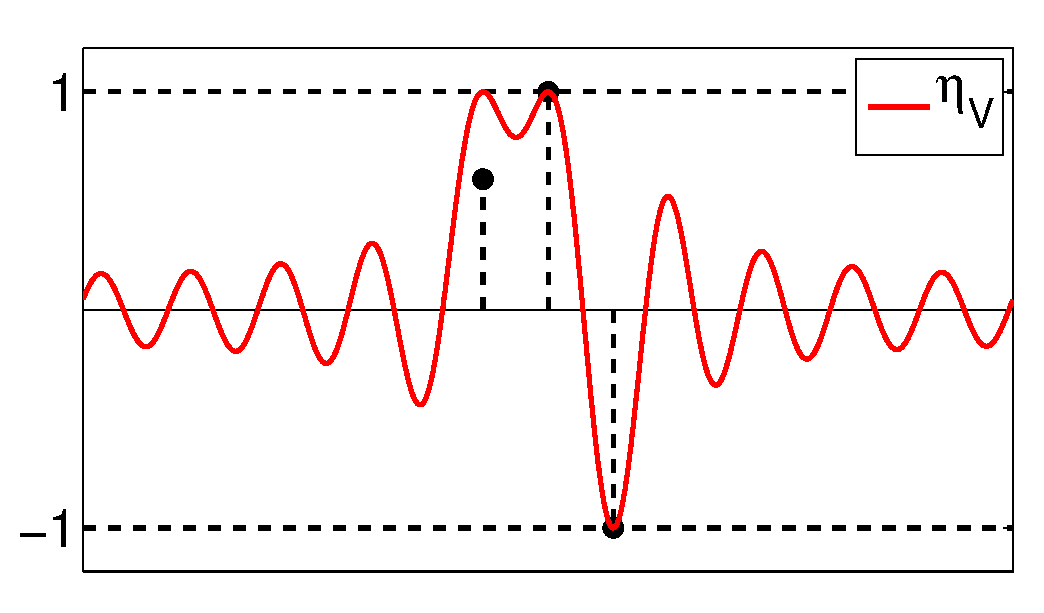
\includegraphics[width=0.48\linewidth,clip,trim=0 -27px 0 0]{paths/3diracsa-fc10-certif}&
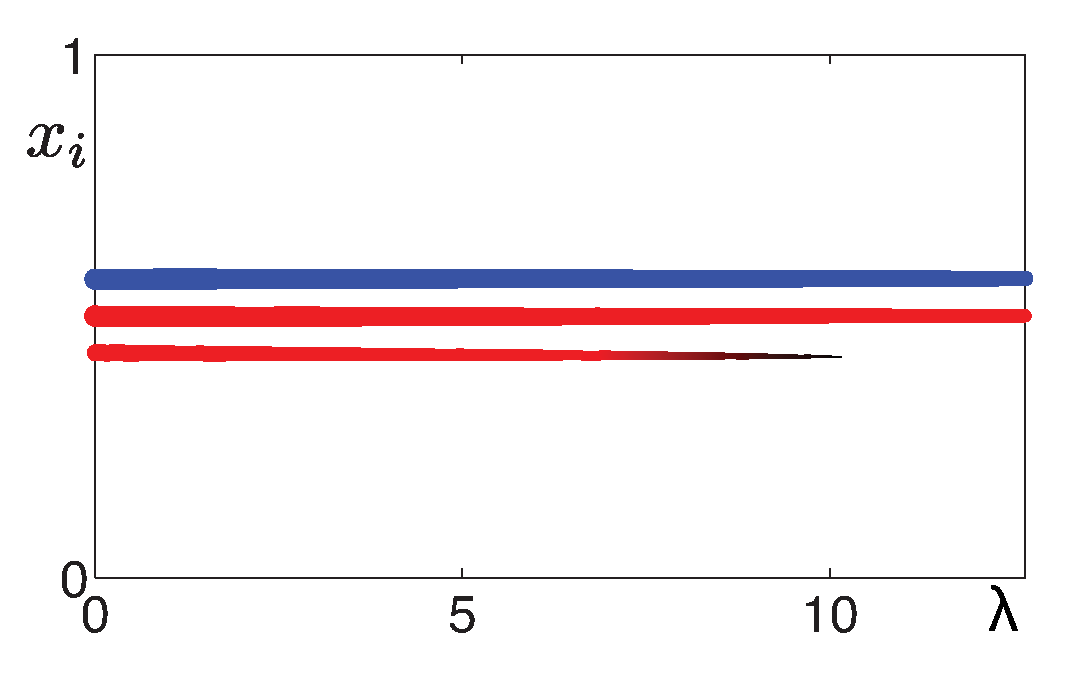
\includegraphics[width=0.49\linewidth]{paths/3diracsa-fc10-noise0-scale0-path}\\
(a) $m_0$ and $\eta_0$ & (b) $w=0$ \\
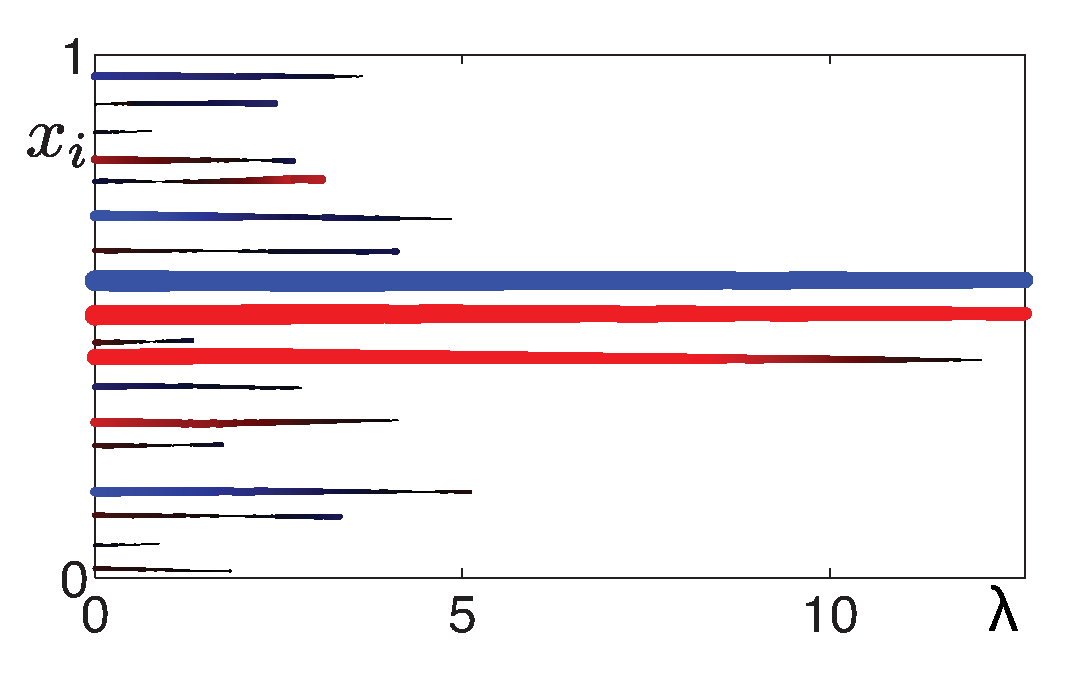
\includegraphics[width=0.49\linewidth]{paths/3diracsa-fc10-noise40-scale0-path}&
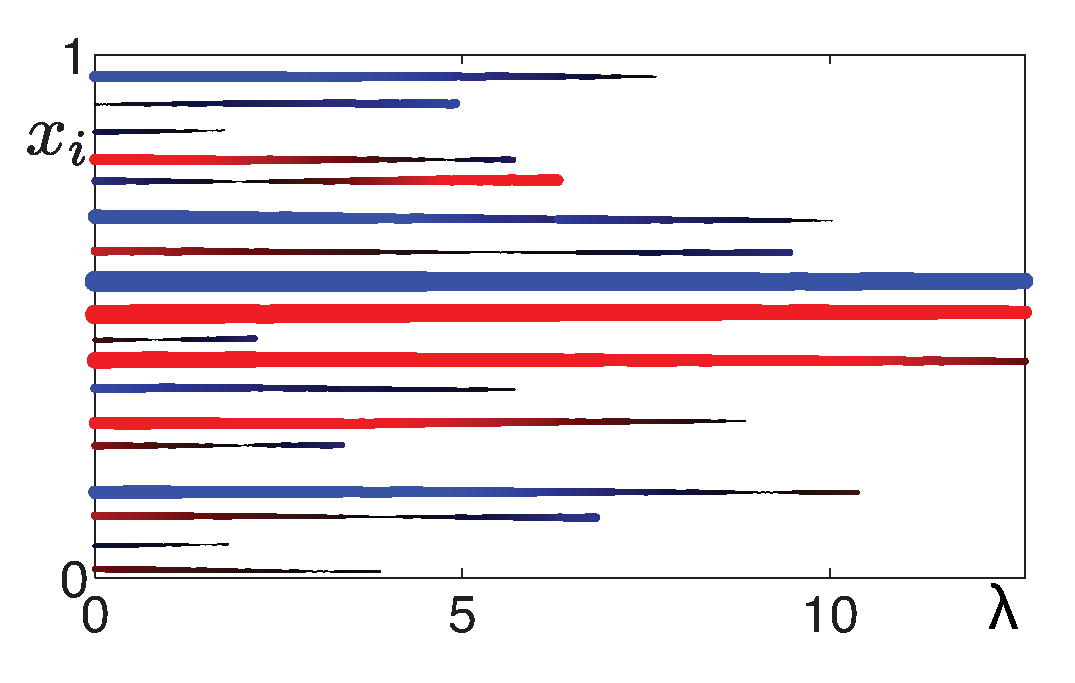
\includegraphics[width=0.49\linewidth]{paths/3diracsa-fc10-noise80-scale0-path}\\
(c) $\norm{w}=0.4 \norm{y}$ & (d) $\norm{w}=0.8 \norm{y}$
\end{tabular}
\caption{\label{fig-paths} 
(a) Input measure $m_0$, and corresponding minimal norm certificate. 
(b,c,d) Regularization paths $\la \mapsto \tilde{m}_\la$ that are solutions of $\Pp_\la(\Phi m_0 + w)$ for three different noise levels $\norm{w}$. 
Each ``strip'' represents the evolution of a spike as $\la$ varies. The color refers to the sign of the spike (blue for negative and red for positive)
and the (vertical) width is proportional to its amplitude.
The exact location is given by the middle of each band.
%The horizontal axis is $\la$, and the vertical axis indexes the Diracs' locations. Each vertical slice of these plots display graphically $m_\la$ with a dot for each Dirac location with a size and color (with blue for negative and red for positive) is proportional to the spike weights.
}
\end{figure} 

As to whether or not the Non Degenerate Source Condition holds for discrete measures, we will discuss this matter in Section~\ref{sec-vanishing} more in depth. For now, let us mention that we have observed empirically that this condition holds under the hypotheses of Theorem~$1.2$ in \cite{Candes-toward}, namely that $\Delta(m)>\frac{1.87}{f_c}$, but also with measures with far smaller values of $\Delta(m)$.


\begin{figure}[htb]
\centering
\begin{tabular}{@{}c@{}c@{}}
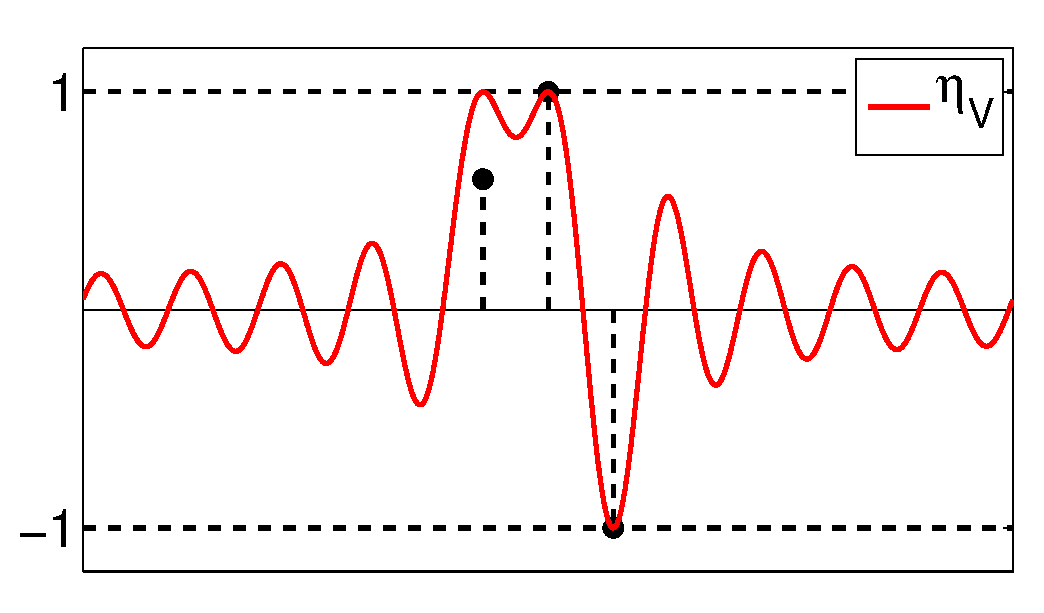
\includegraphics[width=0.48\linewidth,clip,trim=0 -27px 0 0]{paths/3diracsa-fc10-certif}&
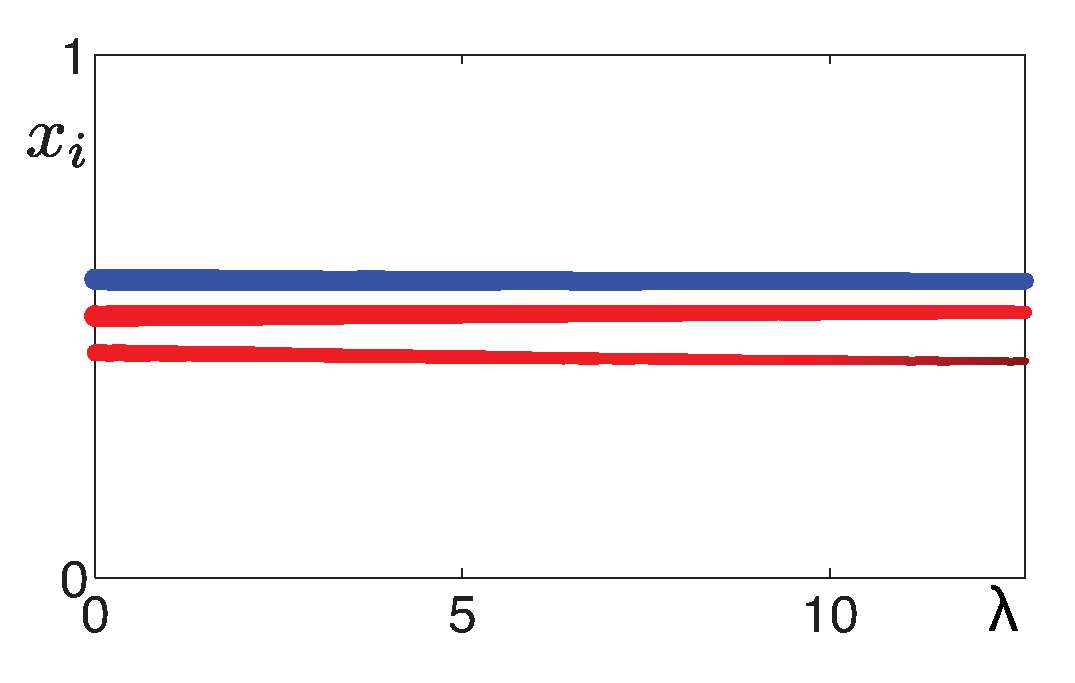
\includegraphics[width=0.49\linewidth]{paths/3diracsa-fc10-noise7-scale1-path}\\
(a) $m_0$ and $\eta_0$ & (b) $\norm{w_0}=0.07 \norm{y}$ \\
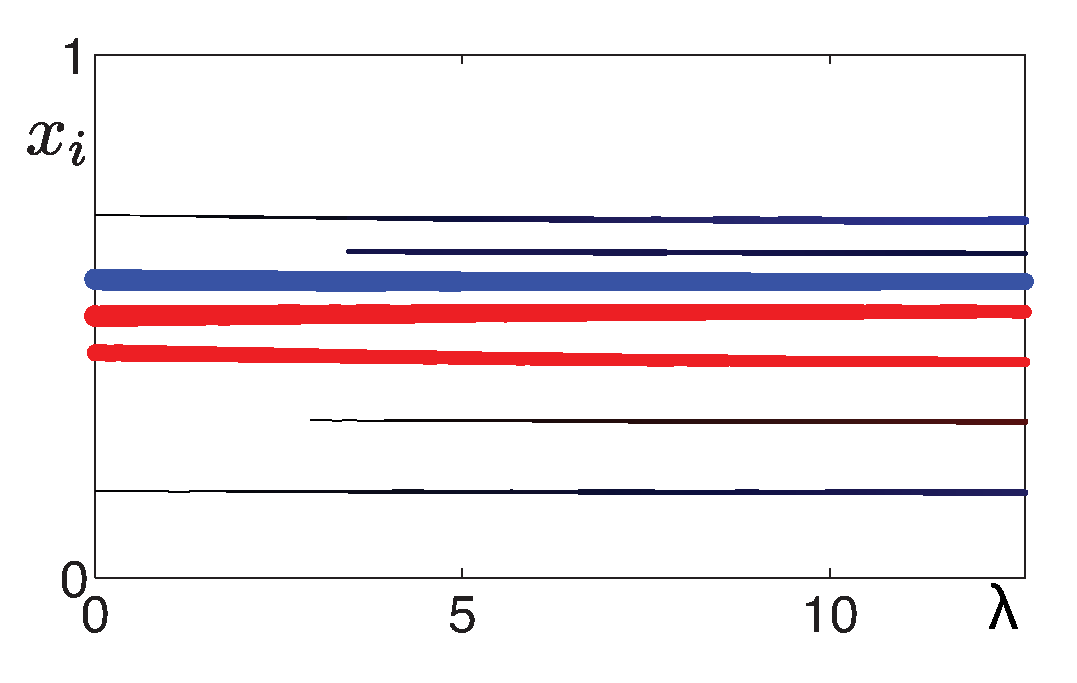
\includegraphics[width=0.49\linewidth]{paths/3diracsa-fc10-noise10-scale1-path}&
\includegraphics[width=0.49\linewidth]{paths/3diracsa-fc10-noise50-scale1-path}\\
(c) $\norm{w_0}=0.1 \norm{y}$ & (d) $\norm{w_0}=0.5 \norm{y}$
\end{tabular}
\caption{\label{fig-paths-scaling} 
Same plots as Figure~\ref{fig-paths} except that the solutions of $\Pp(\Phi m_0 + \la w_0)$ are displayed instead of those of $\Pp_\la(\Phi m_0 + w)$. 
}
\end{figure} 

Figure~\ref{fig-paths} shows the whole solution path $\la \mapsto \tilde{m}_\la$ of the solutions of $\Pp_\la(\Phi m_0 + w)$ when $f_c=10$ and the input measure is identifiable and has three spikes separated by $\Delta(m_0)=0.7/f_c$. Such a measure satisfies the Non-degenerate Source Condition as shown in plot (a). The plots (b,c,d) illustrate the conclusion of Theorem~\ref{thm-noise-robustness}. For values of $\la$ which are too small with respect to $\norm{w}$, the solution $\tilde{m}_\la$ is perturbed with spurious spikes, but as soon as $\la$ is large enough, $\tilde{m}_\la$ has a support that closely (but not exactly) matches the one of $m_0$. For large value of $\la$, spikes starts disappearing, and the support is not correctly estimated. Figure~\ref{fig-paths-scaling} shows the solutions of $\Pp_\la(\Phi m_0 + \la w_0)$, i.e. the noise $w=\la w_0$ is scaled by the regularization parameter $\la$. In accordance with Theorem~\ref{thm-noise-robustness}, this shows that for $\|w\|_2/\la = \|w_0\|_2 \leq 0.07$, the support of the spikes is precisely estimated. 



% Figure~\ref{fig-robust} shows an example of the behavior predicted by Theorem~\ref{thm-noise-robustness}. Here, in order to illustrate Theorem~\ref{thm-noise-robustness}, for each value of $\la$, we have rescaled the noise so that $\norm{w}=\alpha \la$ (with $\alpha=0.7$). The frequency cutoff is $f_c=13$. First, the number of spikes may differ, with some spikes missing or appearing at strange places. But as $\la$ decreases, the number of spikes becomes the same as the original signal, and their positions and amplitudes of the estimated spikes converge to those of the true spikes.
 
% Several animated examples can be downloaded at \url{http://www.ceremade.dauphine.fr/~vduval/spikes.html}.


